\section{Applying Optimizations to SGEMM}
\label{sec:optimization}
The demystified GPU microarchitecture features provides additional space to tune performance-critical kernels. We apply a series of incremental optimizations to improve SGEMM efficiency on Kepler architecture. The optimization strategies go through architectural hierarchy from core and register to memory. All the optimization strategies are inspired by our microbenchmark's observations.
\begin{itemize}
\item At core level, we orchestrate {\tt FFMA} instruction executions by a more efficient instruction scheduling with respect to the proper control code pattern.
\item At register level, we meticulously map operands to registers so that bank conflicts are avoided in the inner loop iteration.
\item At memory level, we select appropriate shared memory load/store width and global memory data path to mitigate latencies.
\end{itemize}

\subsection{Instruction Scheduling}
\subsubsection{Schedule {\tt FFMA} Instructions}
It's unrealistic to keep warp schedulers dual issue the same kinds of arithmetic instructions (i.e., {\tt FFMA}) all the time. Because on Kepler architecture, each warp is assigned a $32$ core privately, $4$ warp schedulers will consume $128$ cores. The reminding $192-128=64$ cores are divided into $2$ groups, each group has $32$ cores, these $32$ cores are shared by $2$ warp schedulers. Two warp schedulers must negotiate who will use the extra $32$ shared cores to avoid resource conflict.
As noted in {\em observation 3}, the best pattern of {\tt FFMA} instructions block is a sequence of $1$ single issue(1 {\tt FFMA}), 2 dual issues (4 {\tt FFMA}s) and 1 single issues ((1 {\tt FFMA})). As shown in Figure~\ref{fig:assemblycode}, the instructions in lines 4-5 and lines 7-8 are respectively grouped as two dual-issues. The other two instructions in line 8 and line 11 are two single issues in terms of floating-point instruction execution. As a comparison, most of the {\tt FFMA}s are single-issues in the CUDA compiler generated codes.

\begin{figure*}[htbp]
\begin{center}
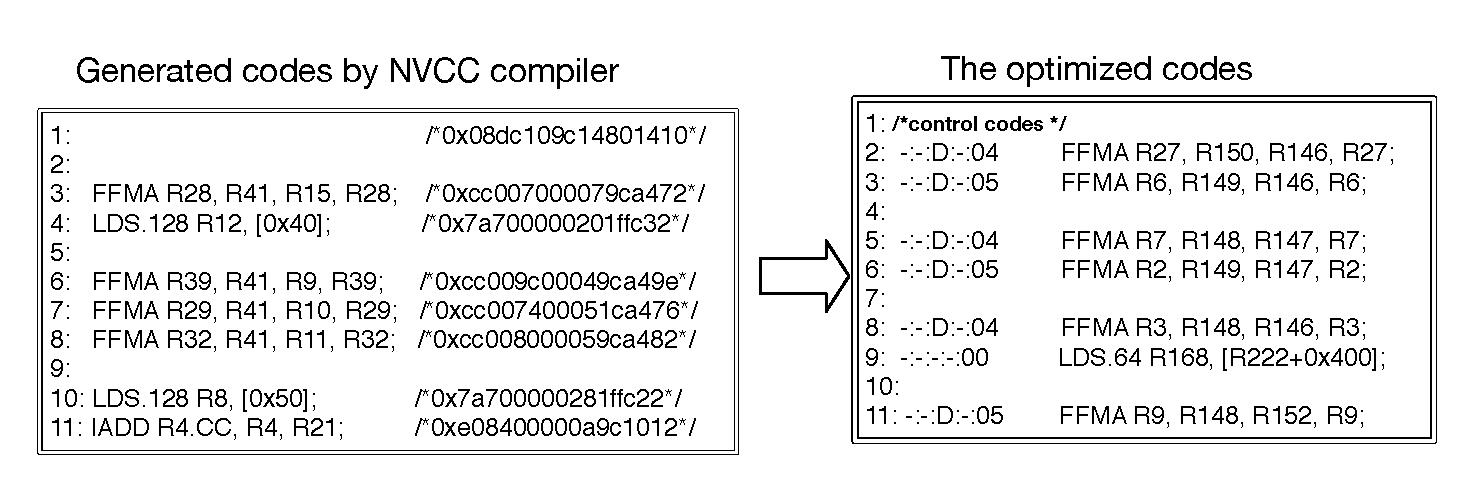
\includegraphics[scale=0.6]{assemlycode}
    \caption{The comparison of compiler generated codes and our tuned assembly codes.}
\label{fig:assemblycode}
\end{center}
\end{figure*}

\begin{figure}[htbp]
\begin{center}
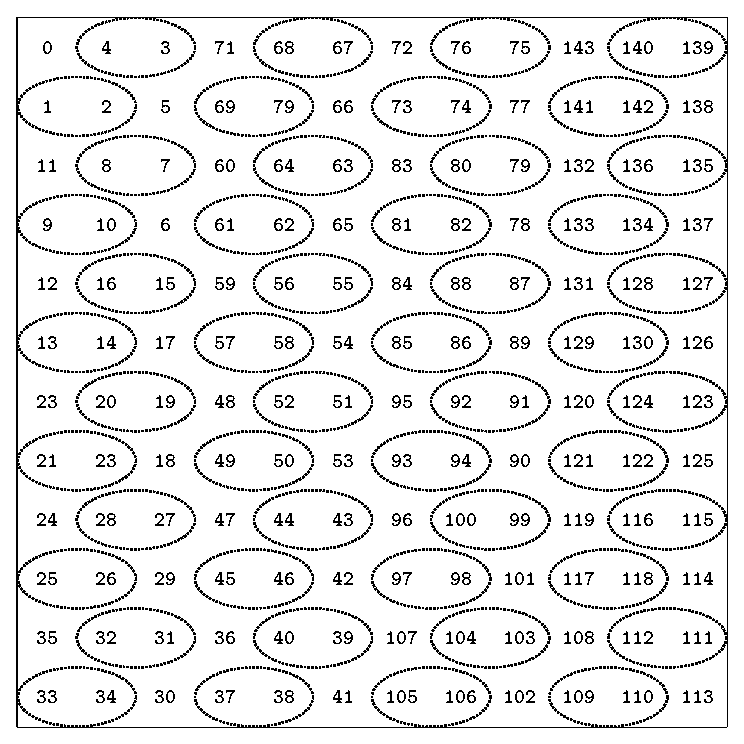
\includegraphics[scale=0.55]{order}
\caption{{\tt FFMA}s instructions scheduling for calculating a $12\times 12$ subblock of matrix C.  The numbers in cells denote {\tt FFMA} execution order. Dashed ellipses across two cells mean that two {\tt FFMA} instructions are executed at same clock cycle.}
\label{fig:order}
\end{center}
\end{figure}

Based on the basic {\tt FFMA} instruction block, the scheduling pattern is depicted in Figure~\ref{fig:order}, which
illustrates the order of $144$ {\tt FFMA}s instruction execution for calculating a $12\times 12$ subblock of matrix C.
For example, the {\tt FFMA} to calculate $c_{00}$ is the first instruction to be issued. Then, both {\tt FFMA}s to
calculate $c_{10}$ and  $c_{11}$ are simultaneously issued. We arrange all the {\tt FFMA} operations according to issue
order illustrated in Figure~\ref{fig:order}.

Another advantage of this execution order is less register pressure due to register data reuse, which can facilitate
operand collector mechanism~\cite{collector}. Operand collector is storage element coupled from register file and
provides inputs to the data path of the processor core for executing an instruction. Operands may be cached and reused
in the subsequent instructions. 
The assembly code in Figure~\ref{fig:assemblycode} lists the instructions to calculate $C_{32},C_{22}, C_{21}, C_{30}, C_{31}, C_{20}$, where are corresponding to the orders of $6,7,8,9,10,11$ in Figure~\ref{fig:reg}. 
With the elaborately designed computing order and register allocation, the reuse happens as follows. The {\tt FFMA} in Line $3$ uses cached operand {\tt R150} of line $2$, Line $3$ and Line $4$ share {\tt R146}. Thus, in dual issue mode {\tt FFMA} of Line $3$ and $4$ need to read 4 registers {\tt R146}, {\tt R27}, {\tt R149}, {\tt R6} instead of $6$ registers. The corresponding bank of these registers are $0,1,3,2$, so no bank conflicts happen.
Similarly, Line 7 uses the cached operand {\tt R149} from the Line 4. In dual issue mode, two {\tt FFMAs} of Line 6 and Line 7 need to read $4$ registers {\tt R148}, {\tt R147}, {\tt R7} and {\tt R2}.

\begin{table}[!t]
\caption{The position table of {\tt Non-FFMA} instructions. The inner-loop is unrolled by 4 times. The first column records slot numbers and the first row represents iteration number.}
\label{tab:position}
\captionsetup{font=scriptsize}
\centering
\scalebox{0.78} {
\begin{tabular}{|c|c|c|c|c|}
\hline
\diagbox[width=4em, height=3em]{slot}{unroll} & 0 &1 &2 &3 \\
    \hline
    5 & ISET P0 & IADD A0 & & XOR smB \\
    \hline
    11 & LDS.64 smA & LDS.64 smA & LDS.64 smA & LDS.64 smA \\
    \hline
    17 & LDS.64 smA & LDS.64 smA & LDS.64 smA & LDS.64 smA \\
    \hline
    23 & LDS.64 smA & LDS.64 smA & LDS.64 smA & LDS.64 smA \\
    \hline
    29 & LDS.64 smA & LDS.64 smA & LDS.64 smA & LDS.64 smA \\
    \hline
    35& IADD K, -4 & IADD A1 & TEXDEPBAR & \\
    \hline
    41 & LDS.64 smB & LDS.64 smB & LDS.64 smB & LDS.64 smB \\
    \hline
    47 & LDS.64 smB & LDS.64 smB & LDS.64 smB & LDS.64 smB \\
    \hline
    53 & LDS.64 smB & LDS.64 smB & LDS.64 smB & LDS.64 smB \\
    \hline
    59 & LDS.64 smB & LDS.64 smB & LDS.64 smB & LDS.64 smB \\
    \hline
    65 & & &STS.64 writeS & ISETP P2 \\
    \hline
    71 & & & & \\
    \hline
    77 & & IADD B0 & & LDG A \\
    \hline
    83 & LDS.64 smA & LDS.64 smA & LDS.64 smA & LDS.64 smA \\
    \hline
    89 &ISETP P3 & & &\\
    \hline
    95 & LDS.64 smA & LDS.64 smA & LDS.64 smA & LDS.64 smA \\
    \hline
    101 & & & STS.64 loadB0 & LDG B \\
    \hline
    107 & & & STS.64 loadB2 & XOR writeS \\
    \hline
    113 & & & & \\
    \hline
    119 & LDS.64 smB & LDS.64 smB & LDS.64 smB & LDS.64 smB \\
    \hline
    125 & & & XOR smA & \\
    \hline
    131 & LDS.64 smB & LDS.64 smB & LDS.64 smB & LDS.64 smB \\
    \hline
    137 & & & & \\
    \hline
    143 & & IADD B1 & BAR.SYNC & BAR Loop \\
    \hline
\end{tabular}
}

\end{table}

\subsubsection{Schedule {\tt non-FFMA} Instructions}

After setting the order of {\tt FFMA}, other {\tt non-FFMA} instructions should be inserted in proper positions to assure
correctness of the program without losing performance. In order to tolerate instruction latency, we need to keep distance of dependent instructions to be larger than the latency. The distance can be approximately computed as
\begin{displaymath}
distance = \frac{4\times\#instructions}{7}
\end{displaymath}
In a schedule block, there are $7$ instructions which cost $4$ clocks to be issued in dual issue mode. In other word, if we want to have interleave
two instructions of $L$ distance, then $\frac{L*7}{4}$ instructions are needed. Besides, the remained number of slots to insert these instructions is estimated as follows:

\begin{displaymath}
\#slots = \frac{rx\times ry\times unroll}{ffmas\_in\_schedule\_block}=\frac{12\times 12\times 4}{6}=24\times 4
\end{displaymath}
In this formula, $rx\times ry\times unroll$ yields total number of {\tt FFMA} for one threads inside register blocking loop.
\jled{the meaning of rx, ry, unroll, and ffmas\_in\_schedule\_block.}
and denominator is {\tt FFMA} instructions inside one schedule block. As stated in section~\ref{sec:benchmark}, the number is $6$ by our $1-2-2-1$ dual issue pattern.
According to these principles, we first arrange {\tt LDS}, {\tt STS}, {\tt LDG} due to their long latencies. The
schedule slots are illustrated in two dimension as shown in Table~\ref{tab:position}.
Note that we use double buffers to hide latency of {\tt LDG} from global memory, which costs $200$ clock cycles.
Every $4$ loop requires $2$ {\tt LDG}s to load data from global memory to registers, $4$ {\tt STS}s to store data from registers to shared memory. There is a read after write (RAW) dependency between {\tt
LDG} and {\tt STS}. The simple model estimates that $\frac{200\times 7}{4} = 350$ are needed instructions between them.
As shown in Table~\ref{tab:position}, we put {\tt LDG} and  {\tt STS} in position $P[77][3]$ and position $P[65][2]$, respectively. Thus, the number of instructions between them are $143-77 + 144\times 2 +
65=419$, resulting in a distance of $\frac{4\times 419}{7}=239$ clocks, which is enough to hide latency of {\tt LDG}s.

The arrangement of {\tt LDS}s, which load data from shared memory for double buffers of both $A$ and $B$, follows the same way with {\tt LDG}s.
A {\tt LDS} has a latency of $40$ clock cycles, $\frac{40\times 7}{4}=70$ instructions are needed to interleave {\tt LDS} and {\tt
FFMA}. As shown in Table~\ref{tab:position}, {\tt LDS} in $P[11][3]$ read data from {\tt STS} in position $P[65][2]$, the distance is more than $40$ clock
cycles. In the end, a {\tt BAR.SYNC} should be inserted after {\tt STS} before {\tt LDS} to make sure that data in shared memory is ready. Other instructions like {\tt XOR},
{\tt IADD}, {\tt ISETP} are inserted according to data dependency, there is almost no performance loss due to little latency.


\subsection{Register Allocation}

To allocate register for $A$ column, $B$ row and $C$ submatrix \jled{explain why?}, we have three considerations: correctness, no bank
conflict and allocate register index tightly.
{\tt LDG.128} restricts $4$ words alignment restriction for register.
Nvidia GPU does not have $128$ bit register, in order to use $128$ bit load, one destination register $RN$ is given, result will be writen to
four $32$ bits registers:{\tt RN}, {\tt RN+1}, {\tt RN+2}, {\tt RN+3}. There is an undocumented restriction: $N\%4==0$, otherwise illegal instruction error will be reported.
It's not hard to understand this restriction, $4$ words alignment for {\tt LDG.128} make hardware logic simpler and cut down power usage.
Since we will use {\tt LDG.128} to load $A$ and $B$, there are $2$ bank allocation choices due to $N\%4==0$ restriction and
bank distribution of Kepler. We assume allocate $A$ matrix bank $\begin{bmatrix} 0 \\ 1  \end{bmatrix}$,
$B$ bank $\begin{bmatrix} 2 & 3 \end{bmatrix}$ as shown in Figure, we have 2 choices left for $C$:
$\begin{bmatrix} 1 & 2 \\ 3 & 0  \end{bmatrix}$
$\begin{bmatrix} 3 & 1 \\ 0 & 2  \end{bmatrix}$.
We have $2\times2$ bank patterns for SGEMM, these four patterns are equivalent in performance, and we arbitrarily choose $\begin{bmatrix} 0 \\ 1  \end{bmatrix}$ $\begin{bmatrix} 2 & 3 \end{bmatrix}$
    $\begin{bmatrix} 1 & 2 \\ 3 & 0  \end{bmatrix}$ for $A$, $B$ and $C$ respectively from the $4$ patterns as shown in Figure~\ref{fig:reg}.
To allocate actual register index, we choose continuous register index so that register index do not get too big to
exceed 255 restriction. From figure, we can verify that $C_{ij}$, $A_i$ and $B_j$ have different banks, for example
$C_{01}$'s color is white, $A_0$'s color is green and $B_1$'s color is red, hence no bank conflicts.

\begin{figure}[htbp]
\begin{center}
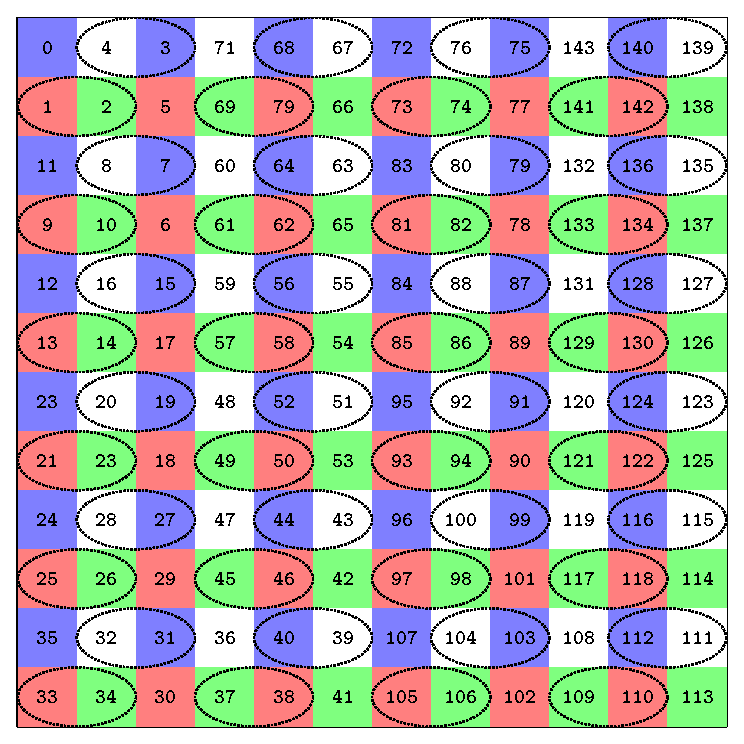
\includegraphics[scale=0.55]{reg}
\caption{An illustration of register bank allocation. The number in the cell is register number.
    The leftmost column of registers are allocated to one column of $A$ sub-matrix, the
top row of registers are allocated to one row of sub-matrix $B$, others are registers for
sub-matrix $C$. The different colors denotes mapping of register banks: Green$\rightarrow$bank0, blue$\rightarrow$bank1, gray$\rightarrow$bank2, red$\rightarrow$bank3.}
\label{fig:reg}
\end{center}
\end{figure}


\subsection{Memory Movement}
According to the optimization observation on memory access suggested by microbenchmark, we use {\tt LDS.64} to load data from shared memory and {\tt LDG.E.128} to load data from global memory. Specifically we have additional reasons to adopt them in SGEMM kernel. First, the use of {\tt LDG.E.128} can reduce the number of {\tt non-FFMA} instructions. For example,  in the inner loop, the number of 32-bits load operations to read $A$ and $B$ is 12. The wider {\tt LDG.E.128} operation reduces the numbers to 3.

Second, it is another story for shared memory. The shared memory transaction size of 256 bytes forces that any shared memory request will be split into multiple transactions of 256 bytes. By inspecting the inner loop, we cannot control when the second transactions happen so that it is difficult to eliminate potential bank conflicts between {\tt LDS.128}s and {\tt FFMA}s. As for {\tt LDS.64}, it's determinable to avoid register bank since a transaction just happens at the position of {\tt LDS.64}.

